\chapter{Arhitektura i dizajn sustava}
		
		Projekt kao cjelina sastoji se od sljedećih podsustava:
		
		\begin{enumerate}
			\item  Web poslužitelja
			
			\item  Web aplikacije
			
			\item  Baze podataka
			
		\end{enumerate}
	
		\textbf{Web preglednik} je program koji omogućuje pregled web-stranica i njihovih multimedijalnih sadržaja. Web preglednik prevodi jezik kojim je Web stranica pisana u jezik razumljiv korisniku te šalje korisničke zahtjeve web poslužitelju.
		
		\textbf{Web poslužitelj} je računalo koje pohranjuje web stranice i sadržaje potrebne za njezin prikaz (primjerice HTML dokumente, CSS stilove, JavaScript datoteke i fotografije). Njegova uloga je povezivanje web preglednika s web aplikacijom kako bi ju učinio dostupnom korisniku.
		
		\textbf{Web aplikacija} je program koji radi na poslužitelju, a izvodi se u web pregledniku kojem pruža grafičko korisničko sučelje. Kada korisnik zatraži izvođenje nekog dijela aplikacije, web preglednik taj zahtjev šalje web poslužitelju. Aplikacija izvodi zadatak na poslužitelju i generira rezultat koji poslužitelj šalje web pregledniku, gdje je rezultat vidljiv korisniku kao odgovor na njegov upit. Web aplikacija je povezana s \textbf{bazom podataka} iz koje dohvaća podatke, a ulogu posrednika u komunikaciji između poslužiteljske i klijentske strane ima REST API.\\
		
		
			
		Programski jezik koji smo odabrali za izradu naše web aplikacije je Java, zajedno s JavaSpring radnim okvirom i React front-end knjižnicom za izgradnju korisničkog sučelja te programskim jezikom TypeScript. Razvojna okruženja u kojima ćemo raditi su Eclipse/IntelliJ te Visual Studio Code.
		
			
		Arhitektura našeg sustava temeljit će se na MVC (Model-View-Controller) obrascu. JavaSpring radni okvir omogućuje korištenje MVC softverske arhitekture te gotove komponente za razvoj web aplikacija. Arhitektura zasnovana na MVC obrascu pruža mogućnost odvajanja pojedinih dijelova aplikacije u zasebne komponente, što omogućuje njihov nezavisan razvoj te na taj način olakšava procese optimiranja i održavanja aplikacije.\\\\
		
		
		\textbf{MVC} obrazac softverske arhitekture sastoji se od:
			\begin{enumerate}
				\item  \textbf{Model} -Sadrži podatke, logike i funkcije ugrađene u program, upravlja njima te kao takva čini središnji dio sustava.
				
				\item  \textbf{View} -Predstavlja prikaz podataka (primjerice obrazac, tablica ili dijagram). Iste podatke je moguće prikazati na više različitih načina.
				
				\item  \textbf{Controller} -Upravlja korisničkim zahtjevima tako što pruža vanjsko sučelje web aplikacije u obliku RESTful web usluge (REST API-ja), prihvaća HTTP zahtjeve, poziva odgovarajuće usluge na sloju usluge te vraća odgovore klijentu u obliku JSON datoteke.\\
			\end{enumerate}
		
				
		\section{Baza podataka}
			
			\noindent Za pohranjivanje podataka koristimo relacijsku bazu podataka, konkretno PostgreSQL. 
			Baza podataka sadrži sljedeće entitete:
				
				\begin{packed_item}
					\item Korisnik
					\item Građanin
					\item Udruga
					\item Mjesto
					\item Životinja
					\item Vrsta
					\item Šetnja
					\item Šetnja Životinja
				\end{packed_item}
		
			\subsection{Opis tablica}
				
				\noindent\textbf{Korisnik}  Ovaj entitet sadržava sve informacije za prijavu Građanina i Udruga u sustav. Sadrži atribute: ID, KorisničkoIme, Email, Slika, Lozinka, BrojMobitela. Ovaj 
				entitet je u \textit{One-To-One} vezi s Građaninom i Udrugom preko atributa ID.
				\begin{longtabu} to \textwidth {|X[6, l]|X[6, l]|X[20, l]|}
					
					\hline \multicolumn{3}{|c|}{\textbf{Korisnik}}	 \\[3pt] \hline
					\endfirsthead
					
					\hline \multicolumn{3}{|c|}{\textbf{Korisnik}}	 \\[3pt] \hline
					\endhead
					
					\hline 
					\endlastfoot
					
					\cellcolor{LightGreen} ID & INT	&  	jedinstveni identifikator korisnika 	\\ \hline
					Korisničko ime	& VARCHAR &  korisničko ime korisnika \\ \hline 
					Email & VARCHAR &  e-mail adresa korisnika \\ \hline 
					Slika & LONGBLOB	&  slika profila korisnika		\\ \hline 
					Lozinka & VARCHAR	&  hash lozinke		\\ \hline 
					Broj mobitela & VARCHAR	&  broj mobitela korisnika		\\ \hline 
					
					
				\end{longtabu}
				
				\noindent\textbf{Građanin}  Ovaj entitet sadržava sve informacije vezane za Građanina. Sadrži atribute: ID, ID korisnika, Ime, Prezime. Ovaj entitet je u \textit{One-To-One} vezi s Korisnikom preko atributa ID korisnika, te u \textit{One-To-Many} vezi sa Šetnjom preko atributa ID.
				\begin{longtabu} to \textwidth {|X[6, l]|X[6, l]|X[20, l]|}
					
					\hline \multicolumn{3}{|c|}{\textbf{Građanin}}	 \\[3pt] \hline
					\endfirsthead
					
					\hline \multicolumn{3}{|c|}{\textbf{Građanin}}	 \\[3pt] \hline
					\endhead
					
					\hline 
					\endlastfoot
					
					\cellcolor{LightGreen} ID & INT	&  	jedinstveni identifikator građanina 	\\ \hline
					\cellcolor{LightBlue} ID korisnika	& INT &  jedinstveni identifikator korisnika (korisnik.ID) \\ \hline 
					Ime & VARCHAR &  ime građanina \\ \hline 
					Prezime & VARCHAR	&  prezime građanina		\\ \hline 
					
					
				\end{longtabu}
			
				\noindent\textbf{Udruga}  Ovaj entitet sadržava sve informacije vezane za Udrugu. Sadrži atribute: ID, ID korisnika, Oib, Ime, Adresa, ID mjesta. Ovaj entitet je u \textit{One-To-One} vezi s Korisnikom preko atributa ID korisnika. Entitet je također u \textit{One-To-Many} vezi sa Šetnjom preko atributa ID, te u \textit{Many-To-One} vezi s Mjestom preko atributa ID mjesta.
				\begin{longtabu} to \textwidth {|X[6, l]|X[6, l]|X[20, l]|}
					
					\hline \multicolumn{3}{|c|}{\textbf{Udruga}}	 \\[3pt] \hline
					\endfirsthead
					
					\hline \multicolumn{3}{|c|}{\textbf{Udruga}}	 \\[3pt] \hline
					\endhead
					
					\hline 
					\endlastfoot
					
					\cellcolor{LightGreen} ID & INT	&  	jedinstveni identifikator udruge \\ \hline
					\cellcolor{LightBlue} ID korisnika	& INT &  jedinstveni identifikator korisnika (korisnik.ID) \\ \hline 
					OIB & CHAR &  OIB udruge\\ \hline 
					Ime & VARCHAR &  ime udruge \\ \hline 
					Adresa & VARCHAR	&  adresa udruge		\\ \hline 
					\cellcolor{LightBlue} ID mjesta	& INT &  jedinstveni identifikator mjesta (mjesto.ID) \\ \hline 
					
					
				\end{longtabu}
			
				\noindent\textbf{Mjesto}  Ovaj entitet sadržava sve informacije vezane za Mjesto. Sadrži atribute: ID, Ime. Ovaj entitet je u \textit{One-To-Many} vezi s Udrugom preko atributa ID.
				\begin{longtabu} to \textwidth {|X[6, l]|X[6, l]|X[20, l]|}
					
					\hline \multicolumn{3}{|c|}{\textbf{Mjesto}}	 \\[3pt] \hline
					\endfirsthead
					
					\hline \multicolumn{3}{|c|}{\textbf{Mjesto}}	 \\[3pt] \hline
					\endhead
					
					\hline 
					\endlastfoot
					
					\cellcolor{LightGreen} ID & INT	&  	jedinstveni identifikator mjesta \\ \hline
					Ime & VARCHAR &  ime mjesta \\ \hline 
					
					
				\end{longtabu}
			
				\noindent\textbf{Životinja}  Ovaj entitet sadržava sve informacije vezane za Životinju. Sadrži atribute: ID, Slika, Opis, Ime, ID vrste, Godina rođenja, Preferirana vrsta šetnje, Spol, ID udruge. Ovaj entitet je u \textit{Many-To-One} vezi s Udrugom preko atributa ID udruge, te s Vrstom preko atributa ID vrste. Entitet je u \textit{Many-To-Many} vezi sa Šetnja Životinja preko atributa ID.
				\begin{longtabu} to \textwidth {|X[6, l]|X[6, l]|X[20, l]|}
					
					\hline \multicolumn{3}{|c|}{\textbf{Životinja}}	 \\[3pt] \hline
					\endfirsthead
					
					\hline \multicolumn{3}{|c|}{\textbf{Životinja}}	 \\[3pt] \hline
					\endhead
					
					\hline 
					\endlastfoot
					
					\cellcolor{LightGreen} ID & INT	&  	jedinstveni identifikator životinje \\ \hline
					Slika	& LONGBLOB &  slika životinje \\ \hline 
					Opis & VARCHAR &  opis životinje \\ \hline 
					Ime & VARCHAR &  ime životinje \\ \hline 
					\cellcolor{LightBlue} ID vrste	& INT &  jedinstveni identifikator vrste (vrsta.ID) \\ \hline 
					Godina rođenja & INT	&  godina rođenja životinje \\ \hline 
					Preferirana vrsta šetnje & VARCHAR & preferirana vrsta šetnje životinje \\ \hline
					Spol & VARCHAR & spol životinje \\ \hline
					\cellcolor{LightBlue} ID udruge & INT & jedinstveni identifikator udruge (udruga.ID) \\ \hline
					
				\end{longtabu}
			
				\noindent\textbf{Vrsta}  Ovaj entitet sadržava sve informacije vezane za Vrstu. Sadrži atribute: ID, Ime, Visina, Težina, Životni vijek, Grupa. Ovaj entitet je u \textit{One-To-Many} vezi sa Životinjom preko atributa ID.
				\begin{longtabu} to \textwidth {|X[6, l]|X[6, l]|X[20, l]|}
					
					\hline \multicolumn{3}{|c|}{\textbf{Vrsta}}	 \\[3pt] \hline
					\endfirsthead
					
					\hline \multicolumn{3}{|c|}{\textbf{Vrsta}}	 \\[3pt] \hline
					\endhead
					
					\hline 
					\endlastfoot
					
					\cellcolor{LightGreen} ID & INT	&  	jedinstveni identifikator vrste \\ \hline
					Ime	& VARCHAR &  ime vrste \\ \hline 
					Visina & VARCHAR &  prosječna visina vrste \\ \hline 
					Težina & VARCHAR &  prosječna težina vrste \\ \hline 
					Životni vijek	& VARCHAR &  prosječni životni vijek vrste \\ \hline 
					Grupa & VARCHAR	&  grupa vrste \\ \hline 
					
				\end{longtabu}
			
				\noindent\textbf{Šetnja}  Ovaj entitet sadržava sve informacije vezane za Šetnju. Sadrži atribute: ID, Trajanje, Početak, Vrsta, ID korisnika. Ovaj entitet je u \textit{Many-To-One} vezi s Građaninom preko atributa ID građanina, te u \textit{One-To-Many} vezi sa Šetnja Životinja preko atributa ID.
				\begin{longtabu} to \textwidth {|X[6, l]|X[6, l]|X[20, l]|}
					
					\hline \multicolumn{3}{|c|}{\textbf{Šetnja}}	 \\[3pt] \hline
					\endfirsthead
					
					\hline \multicolumn{3}{|c|}{\textbf{Šetnja}}	 \\[3pt] \hline
					\endhead
					
					\hline 
					\endlastfoot
					
					\cellcolor{LightGreen} ID & INT	&  	jedinstveni identifikator šetnje \\ \hline
					Trajanje	& INT &  vremensko trajanje šetnje \\ \hline 
					Početak & DATETIME &  vrijeme početka šetnje \\ \hline 
					Vrsta šetnje & VARCHAR &  vrsta šetnje \\ \hline 
					\cellcolor{LightBlue} ID građanina & INT	&  jedinstveni identifikator građanina (građanin.ID) \\ \hline 
					
				\end{longtabu}
			
				\noindent\textbf{Šetnja Životinja}  Ovaj entitet sadržava sve informacije o odnosu Šetnje i Životinje. Sadrži atribute: ID, ID šetnje, ID životinje. Ovaj entitet je u \textit{Many-To-One} vezi sa Šetnjom preko atributa ID šetnje, te u \textit{Many-To-Many} vezi sa Životinjom preko atributa ID životinje.
				\begin{longtabu} to \textwidth {|X[6, l]|X[6, l]|X[20, l]|}
					
					\hline \multicolumn{3}{|c|}{\textbf{Šetnja Životinja}}	 \\[3pt] \hline
					\endfirsthead
					
					\hline \multicolumn{3}{|c|}{\textbf{Šetnja Životinja}}	 \\[3pt] \hline
					\endhead
					
					\hline 
					\endlastfoot
					
					\cellcolor{LightGreen} ID & INT	&  	jedinstveni identifikator šetnje životinje \\ \hline
					\cellcolor{LightBlue} ID šetnje & INT	&  jedinstveni identifikator šetnje (šetnja.ID) \\ \hline 
					\cellcolor{LightBlue} ID životinje & INT	&  jedinstveni identifikator životinje (životinja.ID) \\ \hline
					
				\end{longtabu}
			
			
			\subsection{Dijagram baze podataka}
				\begin{figure}[H]
					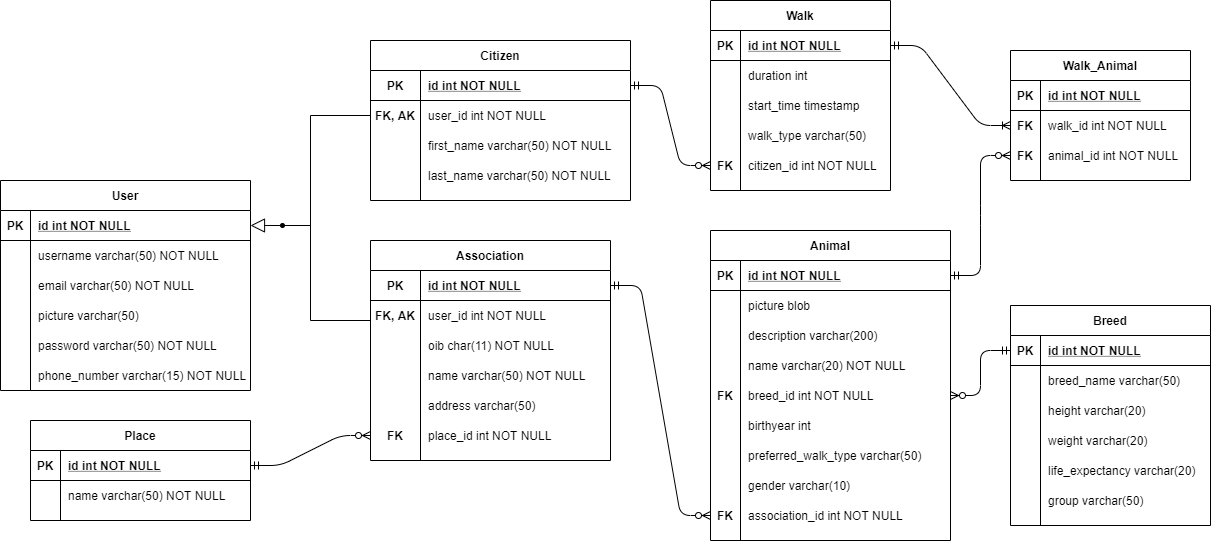
\includegraphics[width=\linewidth]{slike/ERD.png}
					\centering
					\caption{ER dijagram baze podataka}
					\label{fig:erd}
				\end{figure}
			
			\eject
			
			
		\section{Dijagram razreda}
		
			\begin{figure}[H]
				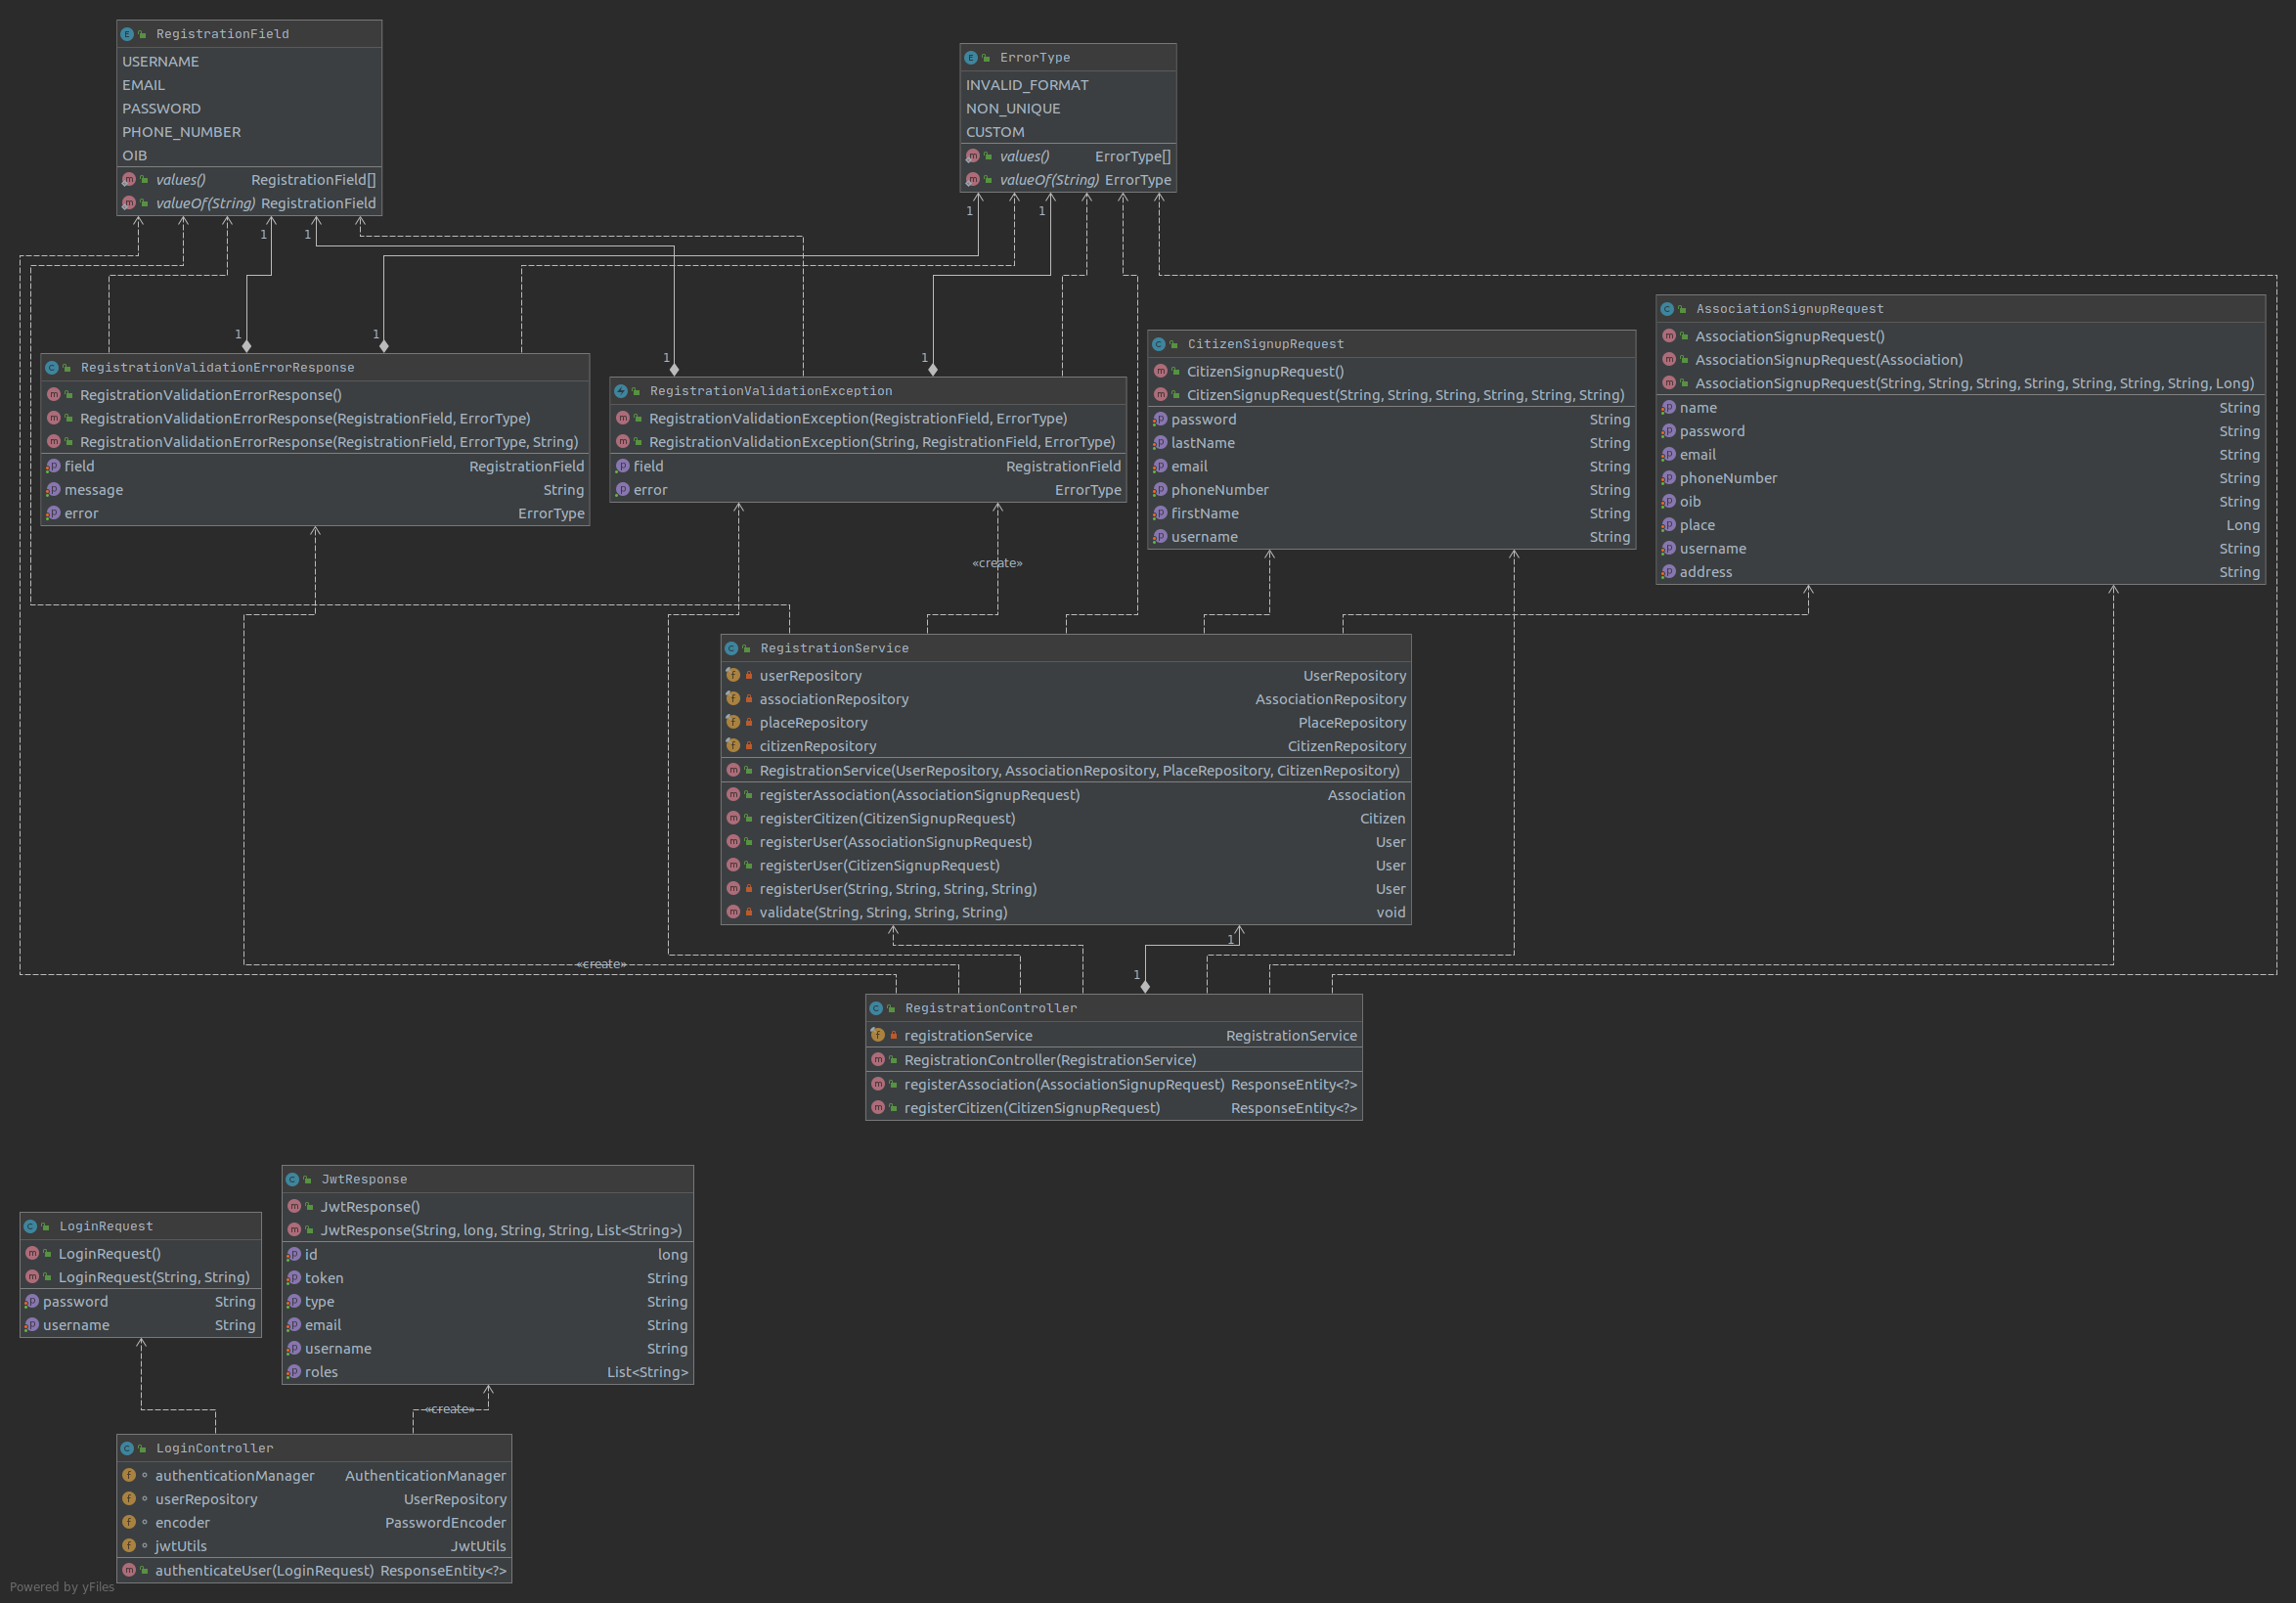
\includegraphics[width=\linewidth]{slike/Controllers-Services-Login-Registration.png}
				\centering
				\caption{Kontroleri i servisi za login i registraciju}
				\label{fig:controllers-services-login-registration}
			\end{figure}
		
			\begin{figure}[H]
				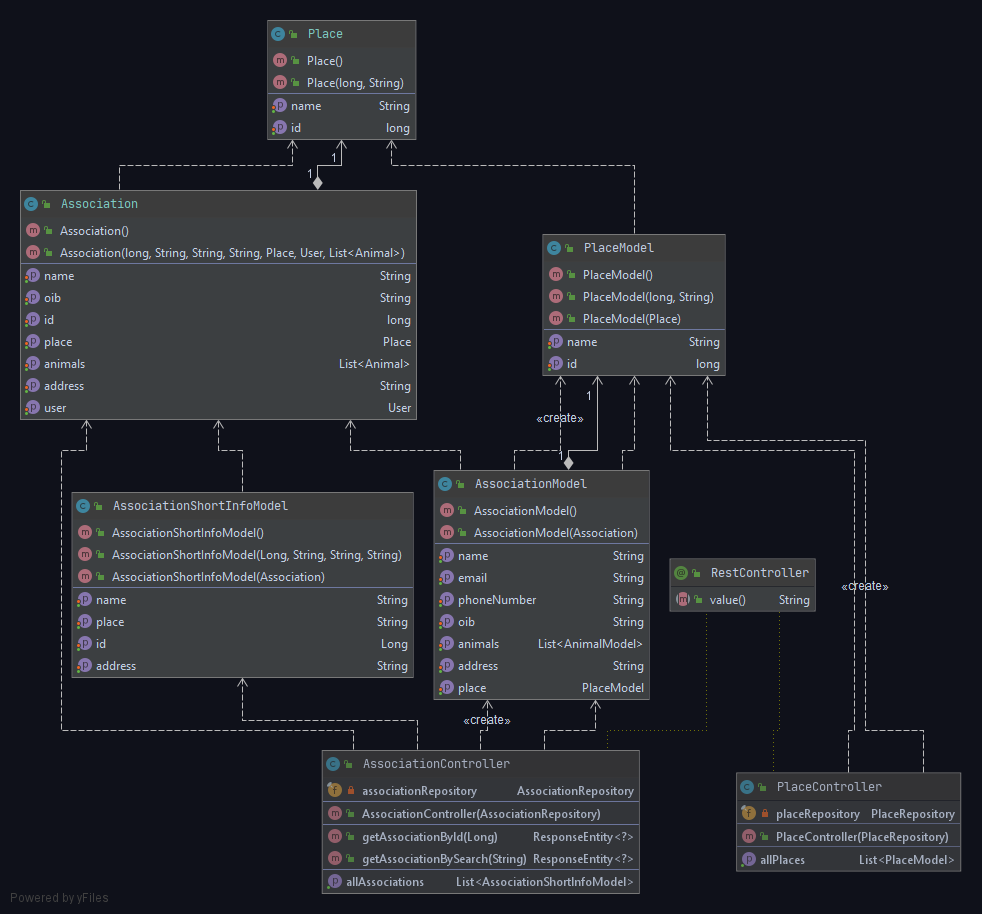
\includegraphics[width=\linewidth]{slike/Controllers-General.png}
				\centering
				\caption{Kontroleri za udruge i mjesta}
				\label{fig:controllers-general}
			\end{figure}
		
			\begin{figure}[H]
				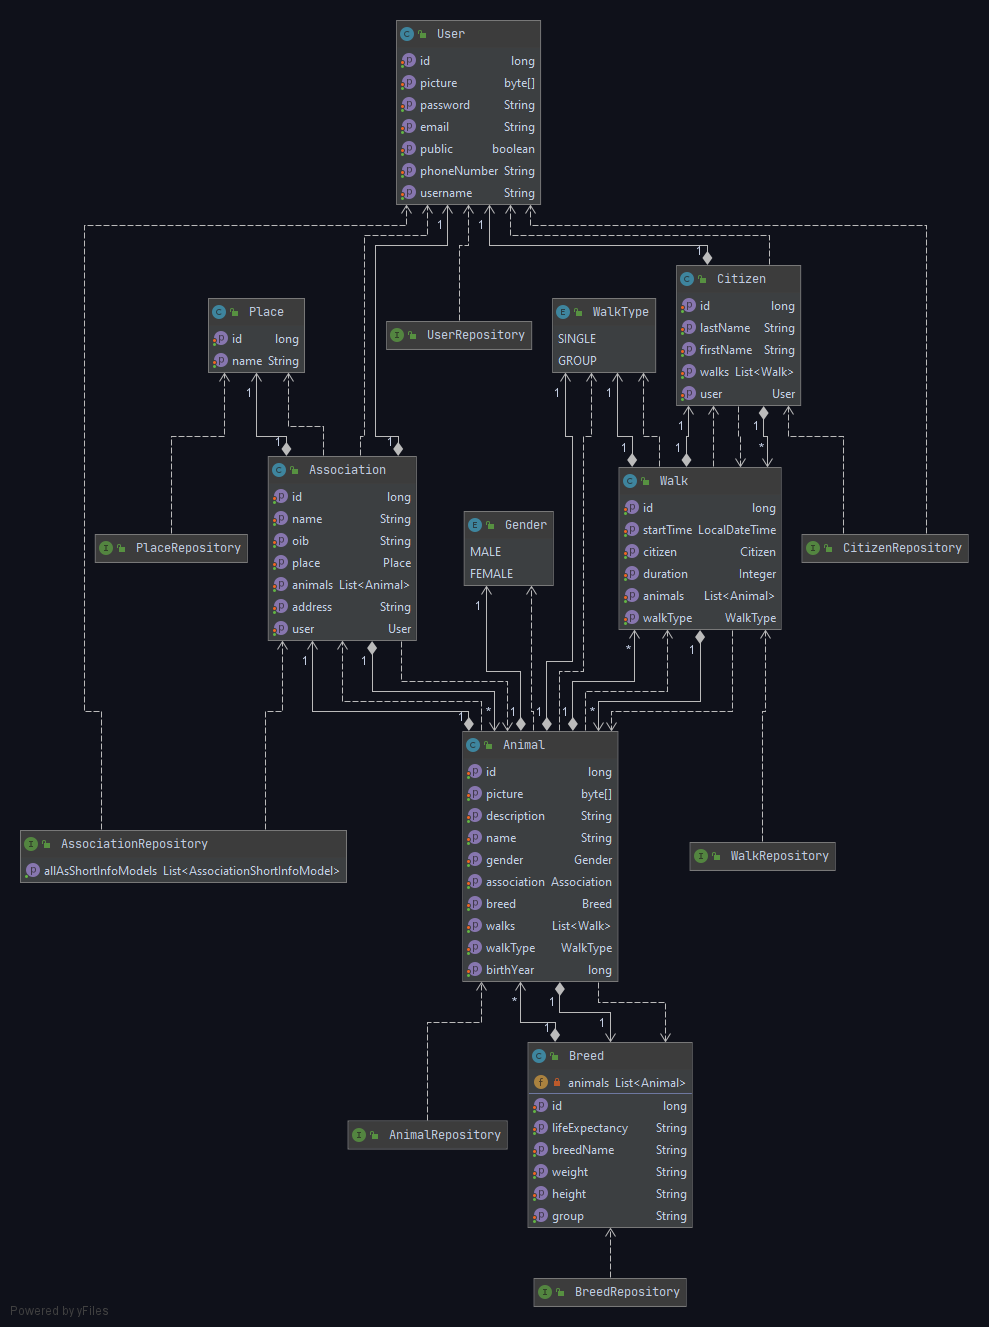
\includegraphics[width=\linewidth]{slike/Entities-Repositories.png}
				\centering
				\caption{Entiteti i repozitoriji}
				\label{fig:entities-repositories}
			\end{figure}
	
			\begin{figure}[H]
				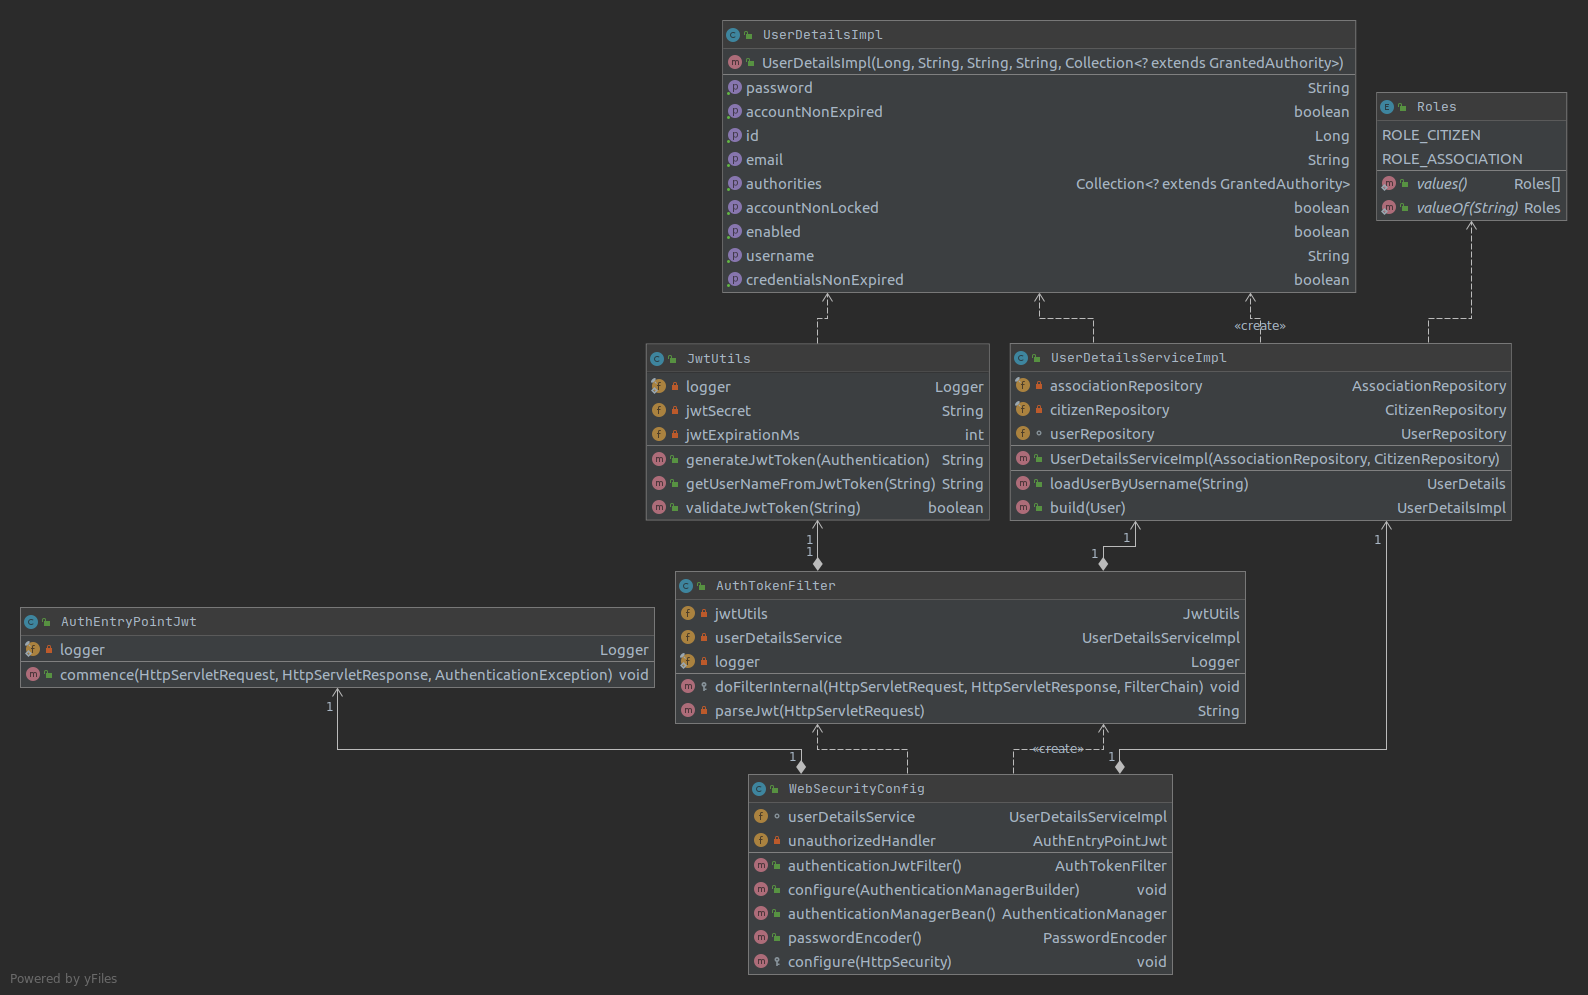
\includegraphics[width=\linewidth]{slike/Security.png}
				\centering
				\caption{Konfiguracija sigurnosti}
				\label{fig:security}
			\end{figure}
			
			\eject
			
			\begin{figure}[H]
				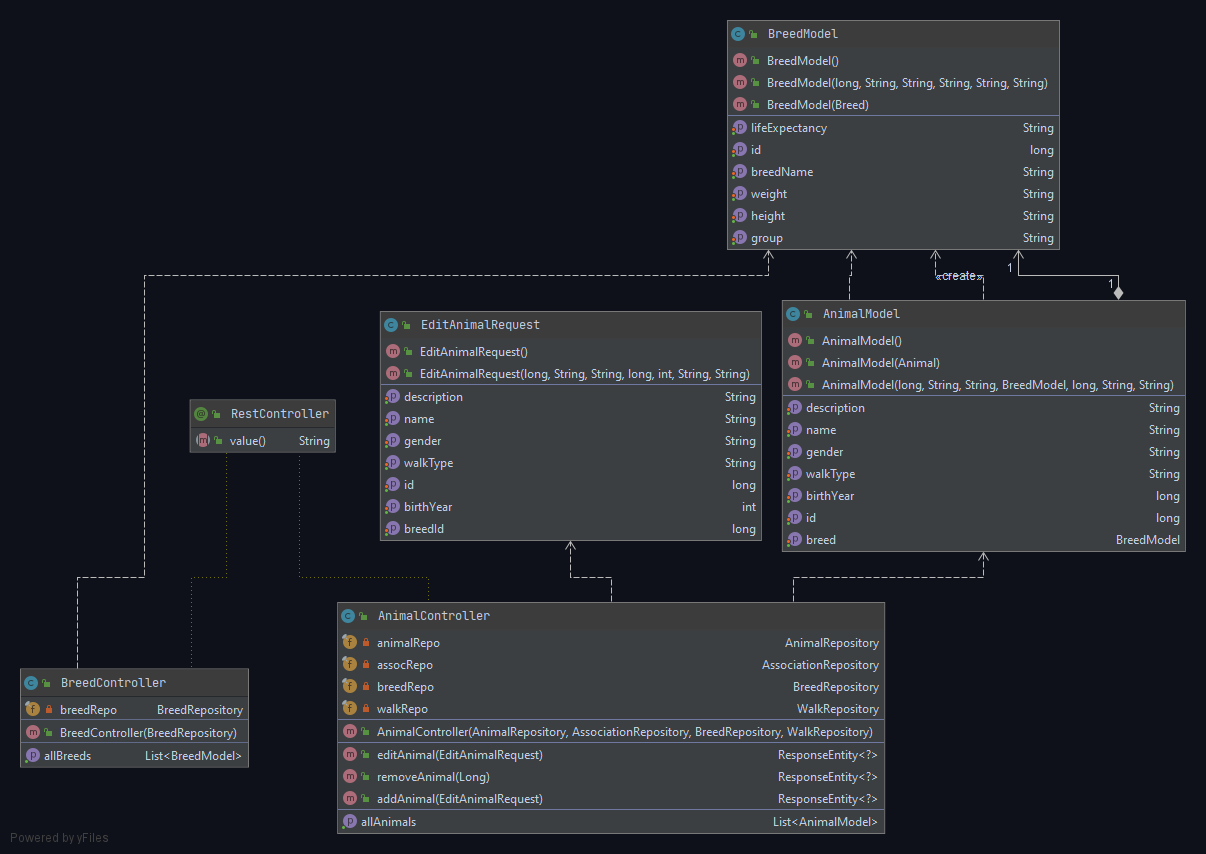
\includegraphics[width=\linewidth]{slike/AnimalController-BreedController.png}
				\centering
				\caption{Kontroleri za životinje i pasmine}
				\label{fig:animalcontroler-breedcontroller}
			\end{figure}
			
			\begin{figure}[H]
				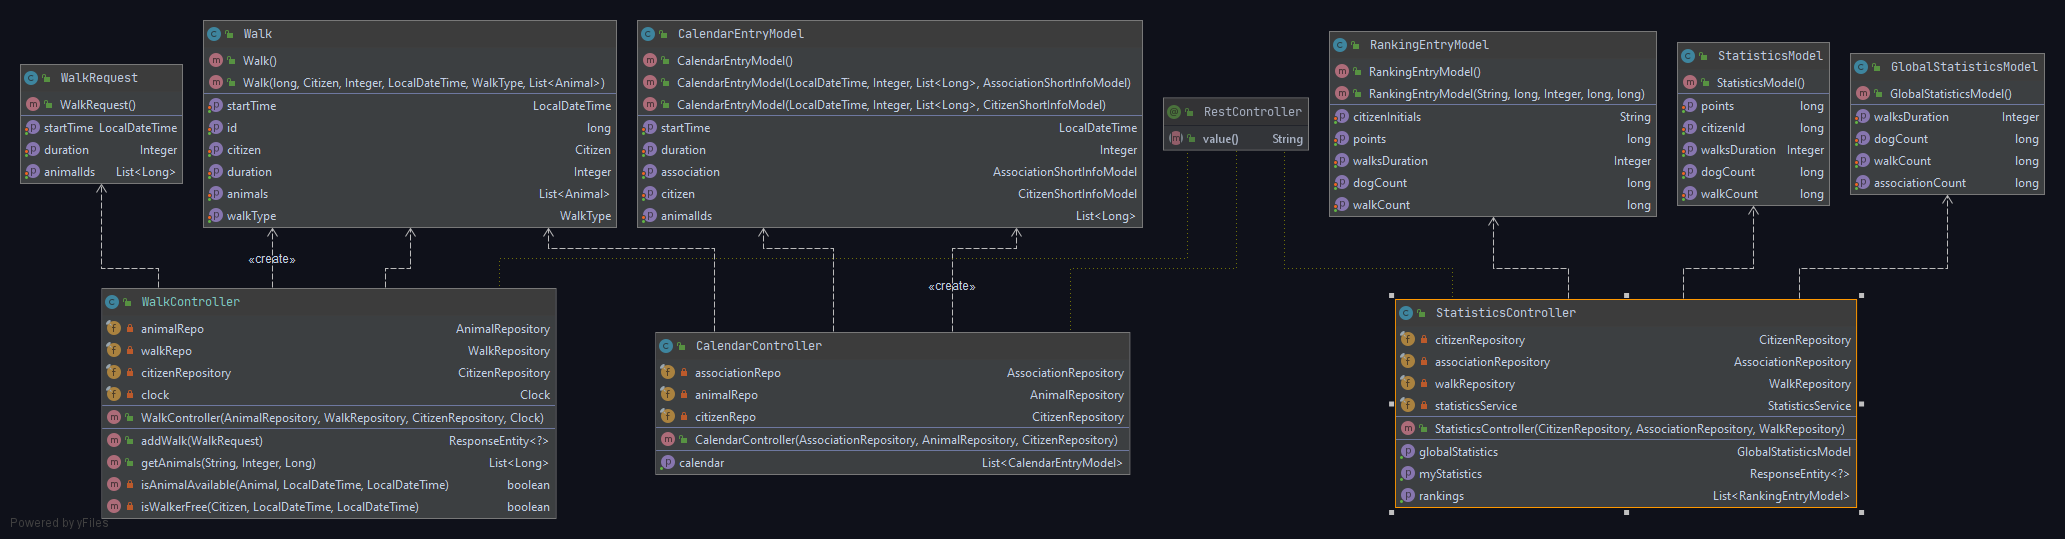
\includegraphics[width=\linewidth]{slike/WalkController-StatisticsController-CalendarController.png}
				\centering
				\caption{Kontroleri za šetnje, statistike i rasporede}
				\label{fig:walkcontroller-statisticscontroller-calendarcontroller}
			\end{figure}
			
			\eject
			
			\section{Dijagram stanja}
			\begin{figure}[H]
				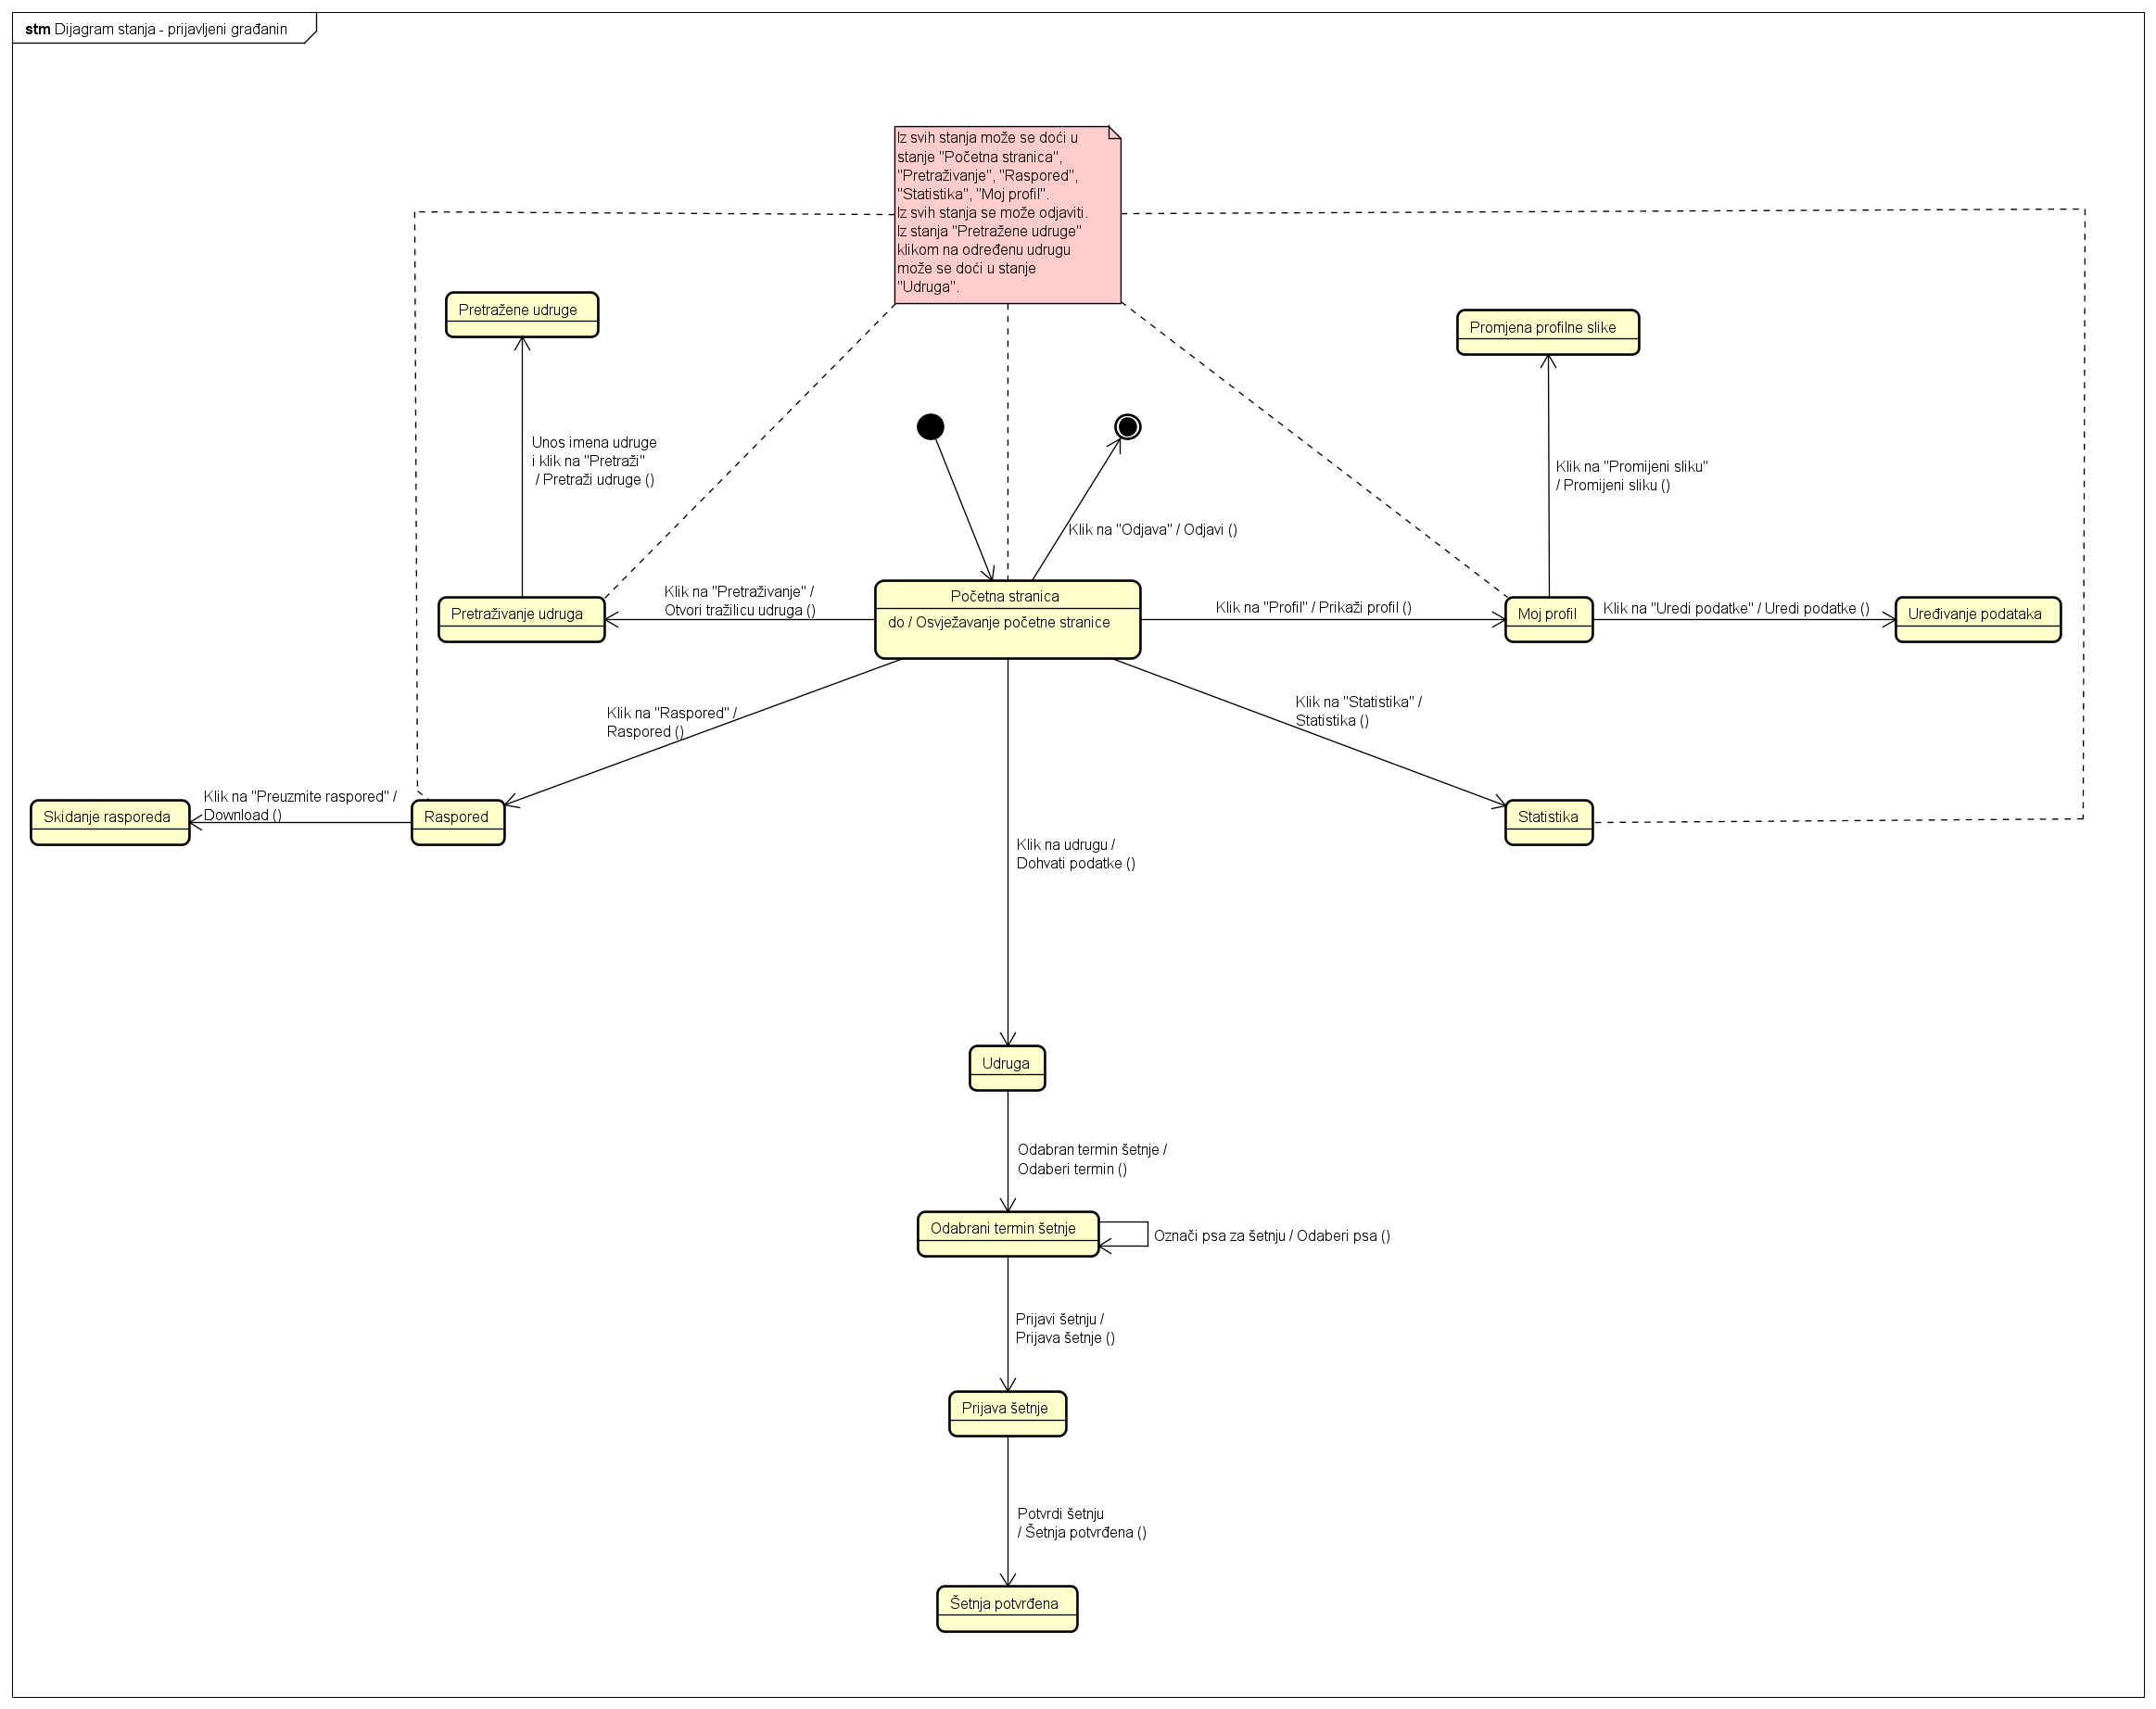
\includegraphics[width=\linewidth]{slike/D_stanja.png}
				\centering
				\caption{Dijagram stanja}
				\label{fig:dijagramstanja}
			\end{figure}
			
			\eject

			\section{Dijagram aktivnosti}
			\begin{figure}[H]
				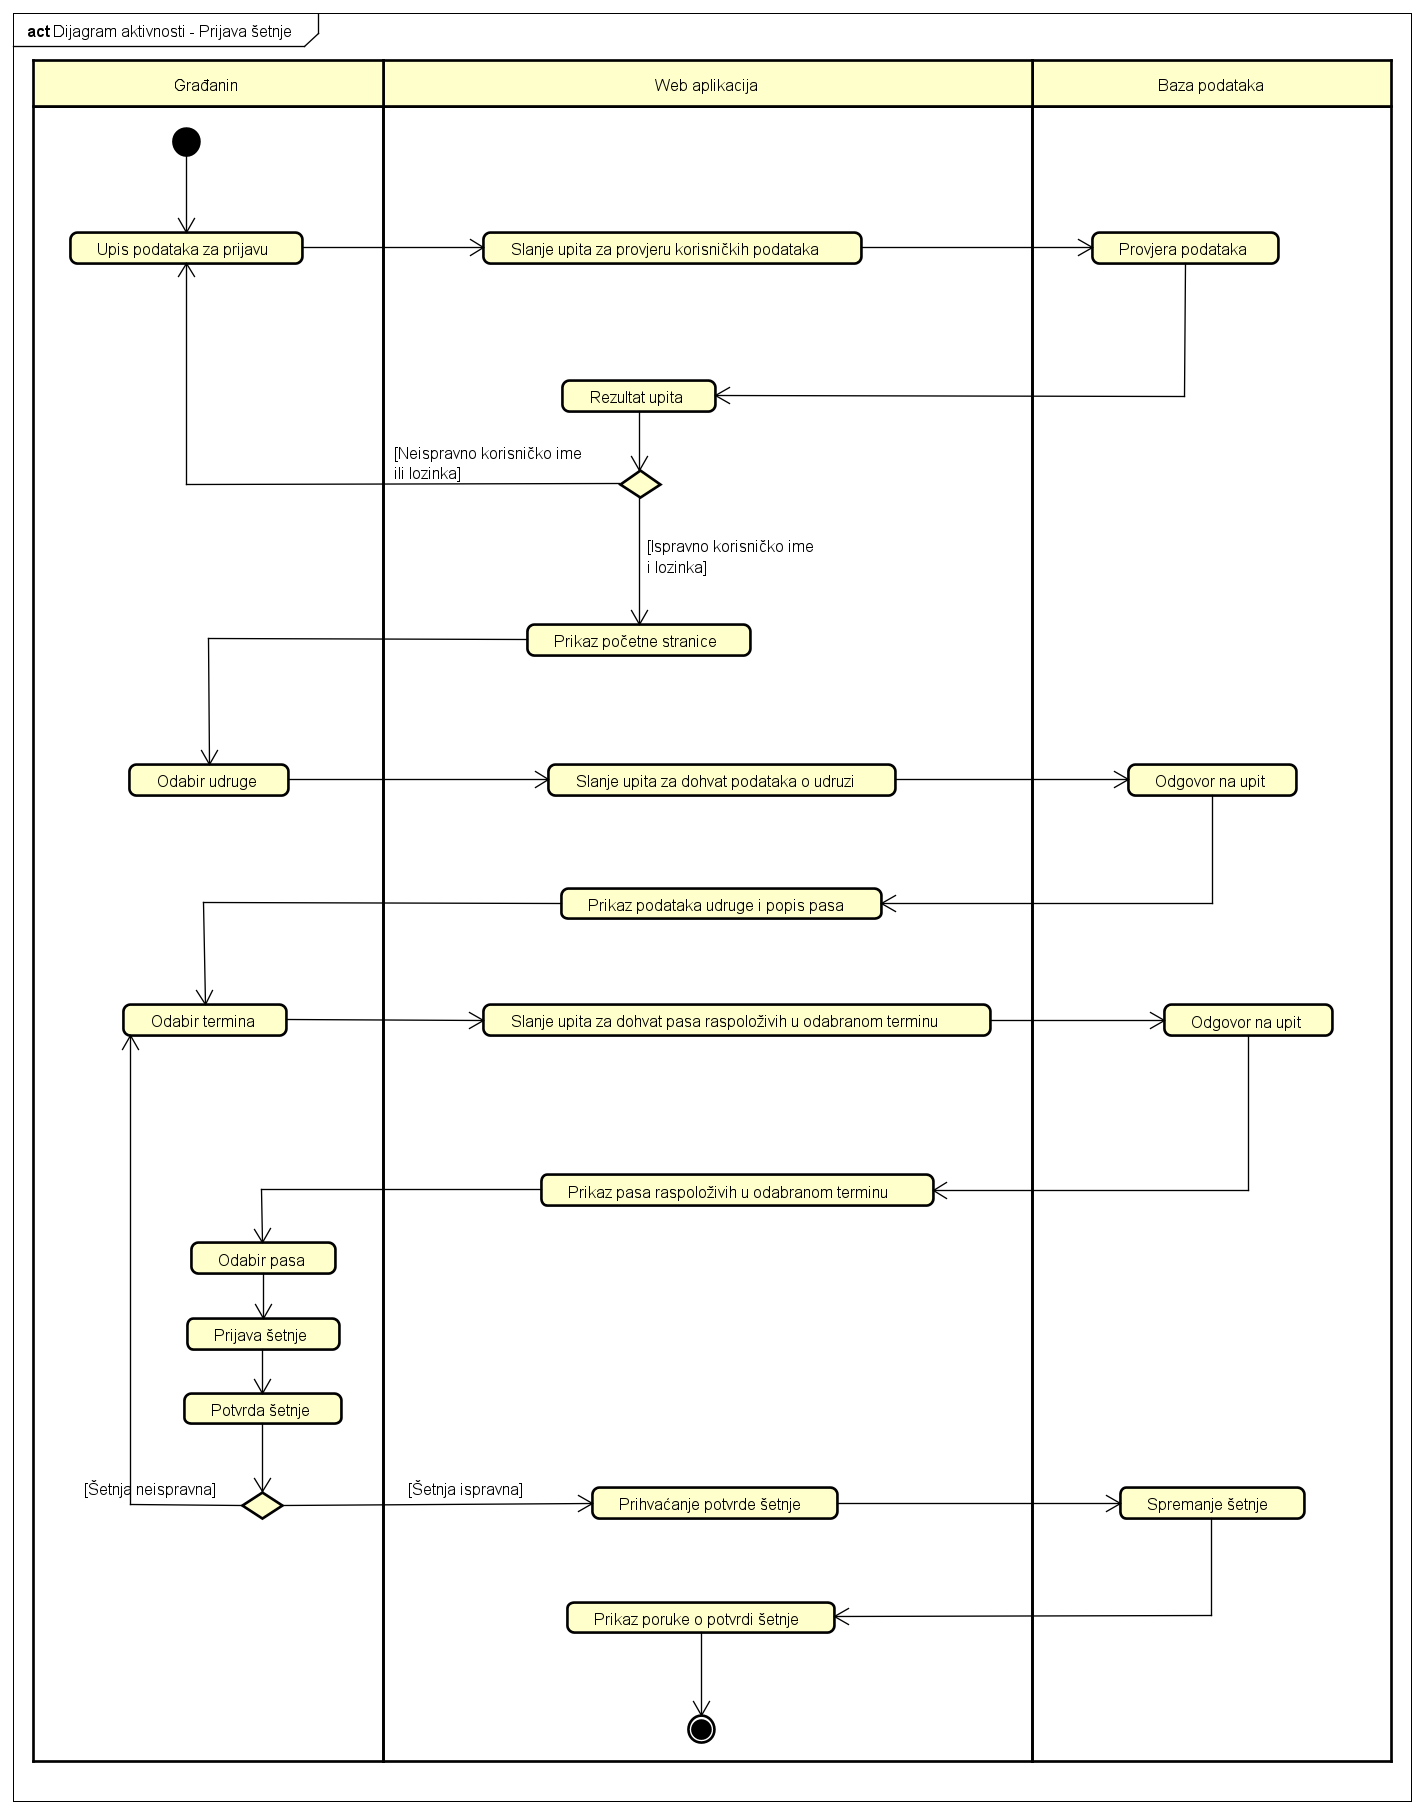
\includegraphics[width=\linewidth]{slike/D_akt.png}
				\centering
				\caption{Dijagram aktivnosti}
				\label{fig:dijagramaktivnosti}
			\end{figure}
			
			\eject
			
			\section{Dijagram komponenti}
			\begin{figure}[H]
				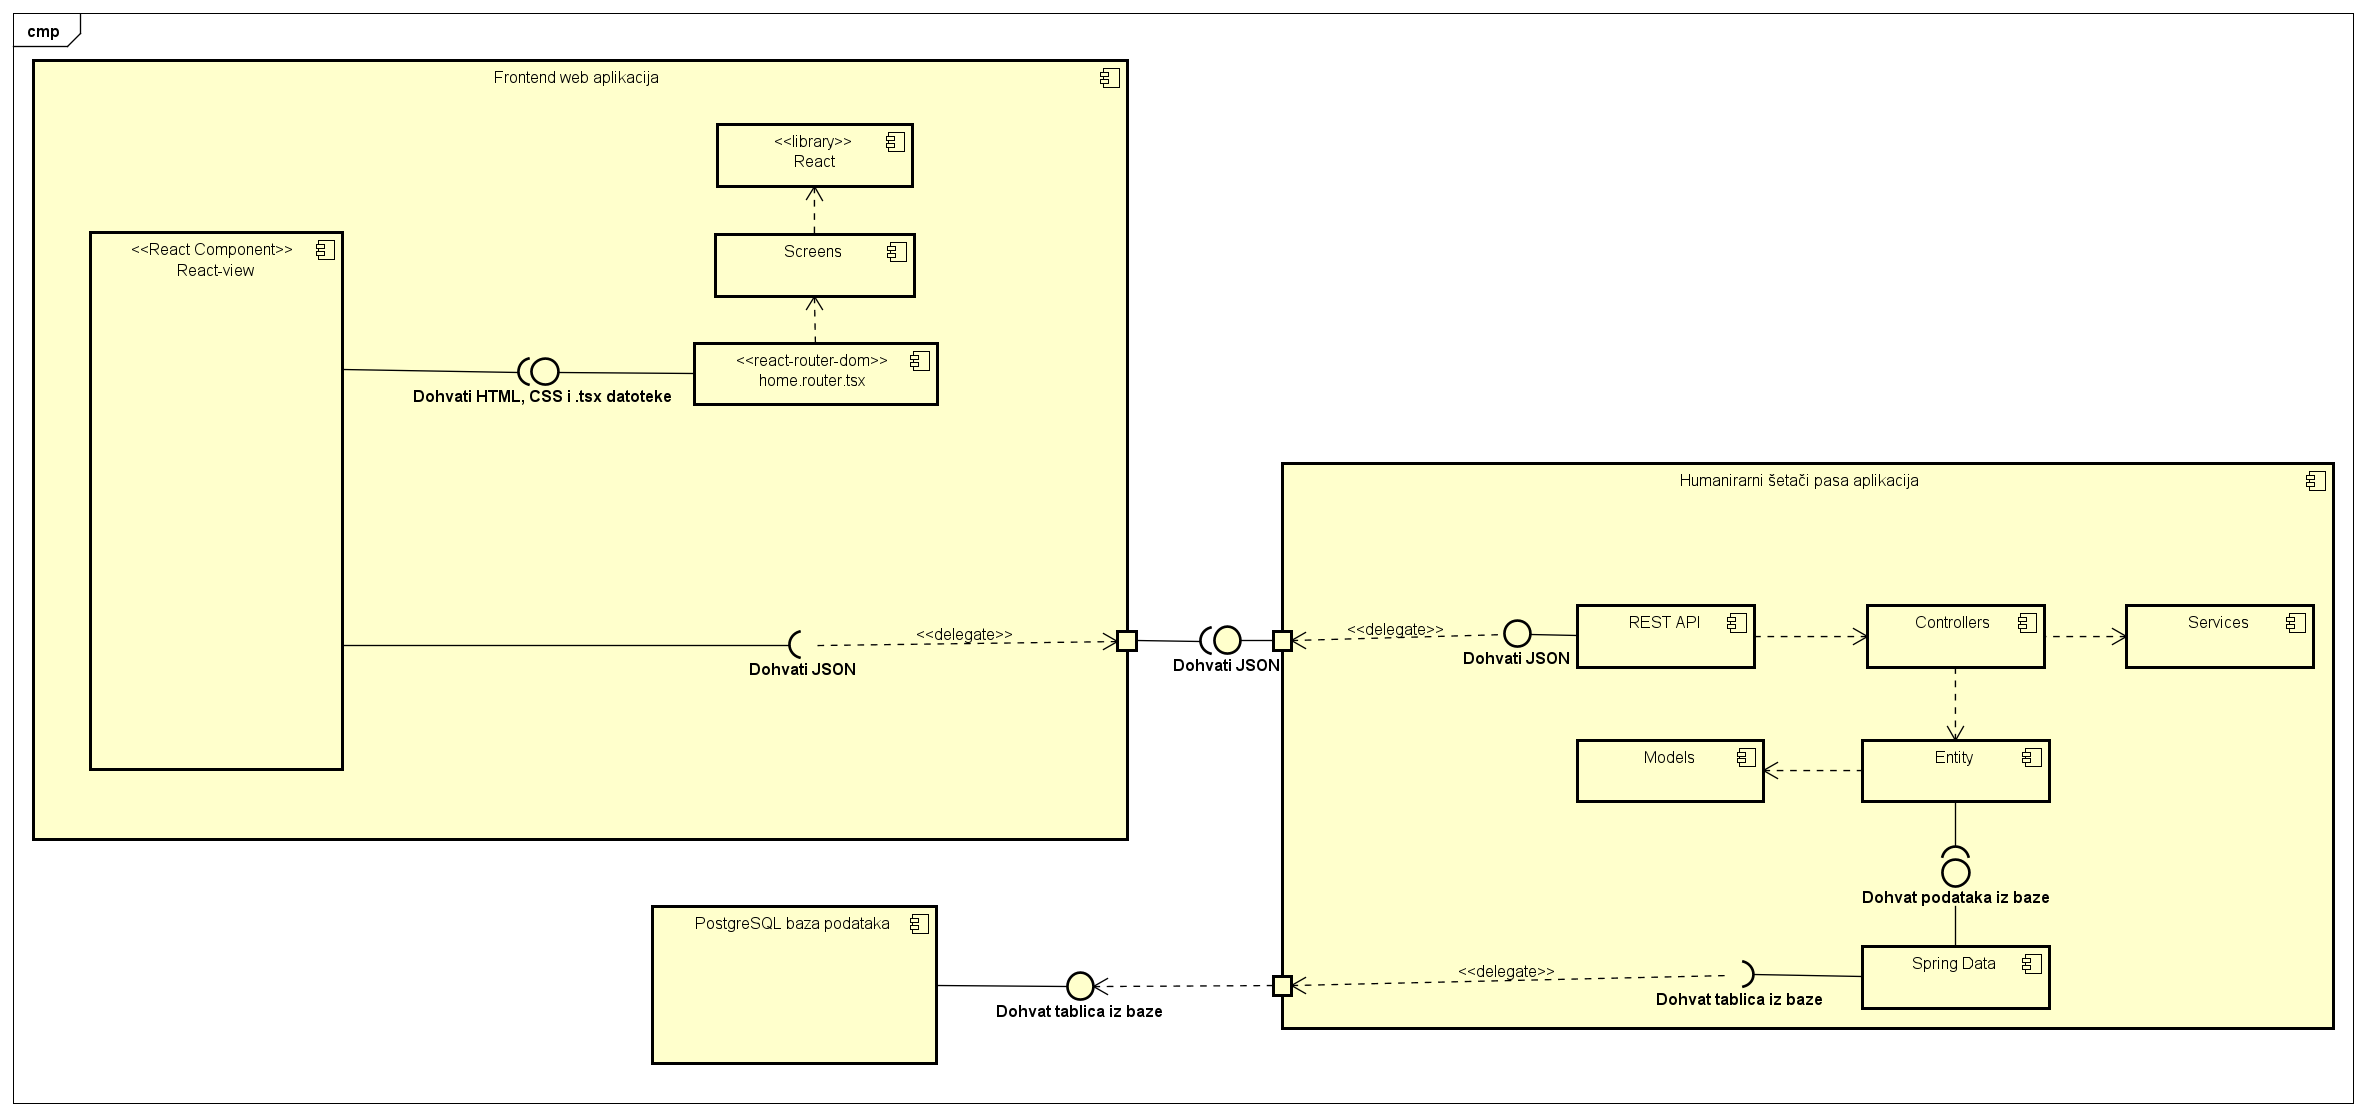
\includegraphics[width=\linewidth]{slike/ComponentDiagram3.png}
				\centering
				\caption{Dijagram komponenti}
				\label{fig:dijagramkomponenti}
			\end{figure}
